\section{Methodology}\label{sec:methodology}
Since this research project aims at performing physical radiation tests, four experiment segments are discussed within this section. \cref{subsec:algorithm} motivates the selected algorithm used for testing. \Cref{subsec:hardware} discusses the hardware that is used and how the radiation effects simulated. The brain adaptation implementations are presented in \cref{subsec:brain_adaptation}. The test method is specified in \cref{subsec:testing}.

\subsection{Algorithm Selection}\label{subsec:algorithm}
The application should be representative of space applications, and it should facilitate application of brain adaptations. This intersection may be image segmentation and or classification using (deep) neural networks. For example, the Mars Organic Molecule Analyzer (MOMA) of ExoMars Rosalind Franklin Rover (scheduled for launch in 2023) will perform rock sample analysis using trained AI systems \cite{}%https://ntrs.nasa.gov/api/citations/20210022097/downloads/AI%20in%20Aerospace%201.pdf. 
Since such systems are typically complex and dependent on large datasets with long training times, this project starts with a more controllable test-environment. Training times and reliance on external datasets are eliminated by opting for graph algorithms that do not require neural networks in Von Neumann form. Within the graph algorithms, some SNN algorithms may be naturally more robust than others. For example, SNN algorithms that calculate the shortest path within graphs may automatically re-route if radiation imposed neuron-death occurs. However, since this research aims at determining the effectivity of brain adaptation mechanisms, a stricter test is found in algorithms that can fail to produce meaningful output if a single neuronal or synaptic property is changed. Therefore, the minimum dominating set (MDS) approximation as presented by Alipour et al, is selected \cite{} for to build the initial brain adaptation implementations. It is specified in\cref{alg:alipour}.
\begin{algorithm}%[1]
    \caption{Distributed Algorithm for computing a total dominating set in a graph with given integer $m\geq 0$.}\label{alg:alipour}
    \KwData{Connected, planar, triangle-free graph of size $n$.}
    \KwResult{Set of nodes that form a minimum total dominating set (MDTS).}
    In the first round, each node $v_i$ chooses a random number $0<r_i<1$ and computes its weight $w_i=d_i+r_i$ and sends $w_i$ to its
    adjacent neighbours.\;
    In the second round, each node $v$ marks a neighbour vertex $v_i$ whose weight $w_i$ is maximum among all the other neighbours of $v$.\;
    \For{$m$ rounds}{
        Let $x_i$ be the number of times that a vertex is marked by its neighbour vertices, let $w_i=x_i+r_i$\;
        Unmark the marked vertices.\;
        Each vertex marks the vertex with maximum $w_i$ among its neighbour vertices.\;
    }
    8: The marked vertices are considered as the vertices in our total dominating set for $G$.\;
\end{algorithm}

Next, an SNN implementation of this algorithm is generated using Leaky-Integrate-and-Fire (LIF) neurons. This implementation is created by Diehl et al. \cite{} using the open source lava software framework by Intel. This implementation takes in connected, triangle-free, planar graphs (E.g. \cref{fig:input_graph}) in the form of networkx objects. Then it converts these graphs into the specification of an SNN that is encoded in a new networkx graph (E.g. \cref{fig:encoded_snn}). A recursive method then takes a single neuron and converts the SNN encoded in the networkx graph, into an actual SNN that can be run on the Loihi (1 \& 2) chips, or simulated on a regular computer.
\begin{figure}[H]
    \centering
    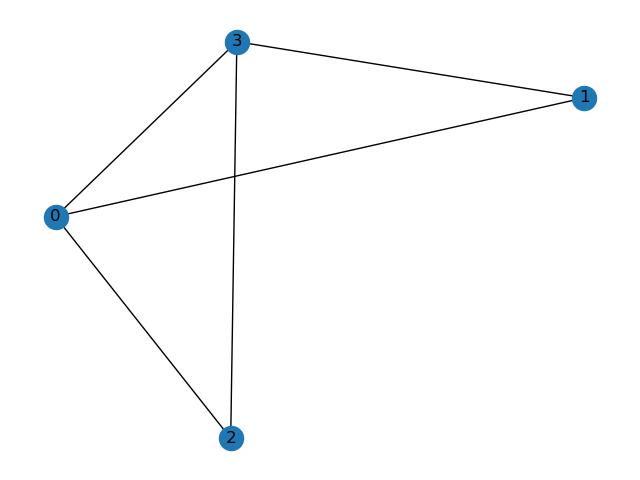
\includegraphics[width=8cm]{latex/Images/input_graph.png}
    \caption{Example input graph. TODO: change to triangle free planar graph.%TODO:
    }
    \label{fig:input_graph}
\end{figure}

\begin{figure}[H]
    \centering
    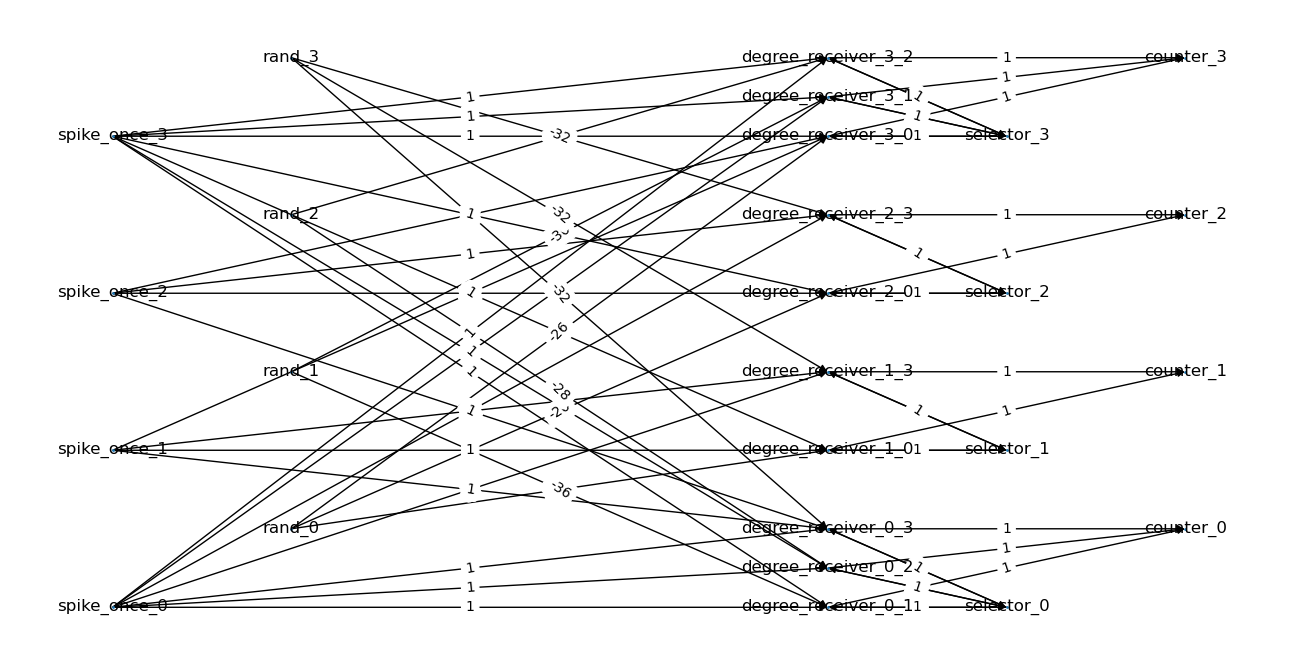
\includegraphics[width=8cm]{latex/Images/structured_graph.png}
    \caption{Example SNN encoding of algorithm to approximate MDS on the input graph of \cref{fig:input_graph}. This module is connected in series where the mark counter neuron takes up the role of spike\_once neuron in the next round of the approximation algorithm. For a more detailed description of the SNN implementation the reader is referred to Diehl et al., or to the source code documentation \cite{}. %TODO: include citation. %TODO: update to match updated input graph.
    }
    \label{fig:encoded_snn}
\end{figure}

\subsection{Hardware}\label{subsec:hardware}
Since at the time of writing no single-event effect (SEEs) propagation mechanisms are identified for space radiation exposure on the Loihi 1 \& 2 chips, a high-level software simulation of these single-event effects is performed. This is done by assuming the non-neuromorphic components of the chips are performing nominally, and that the SEEs propagate from for example transient bit-flips towards neuronal and synaptic parameter changes. The first assumptions may be accurate if local radiation hardening and redundancy is applied to the non-neuromorphic components. Weight and/or energy saving could be a motivation to apply these radiation counter-measures sparsely. The second assumption is based on the digital nature of the components that make up the neural components of the Loihi. The components that make up the neural compartments and synapses of the Loihi are visualised in \cref{fig:loihi_micro_architecture}.
\begin{figure}[H]
    \centering
    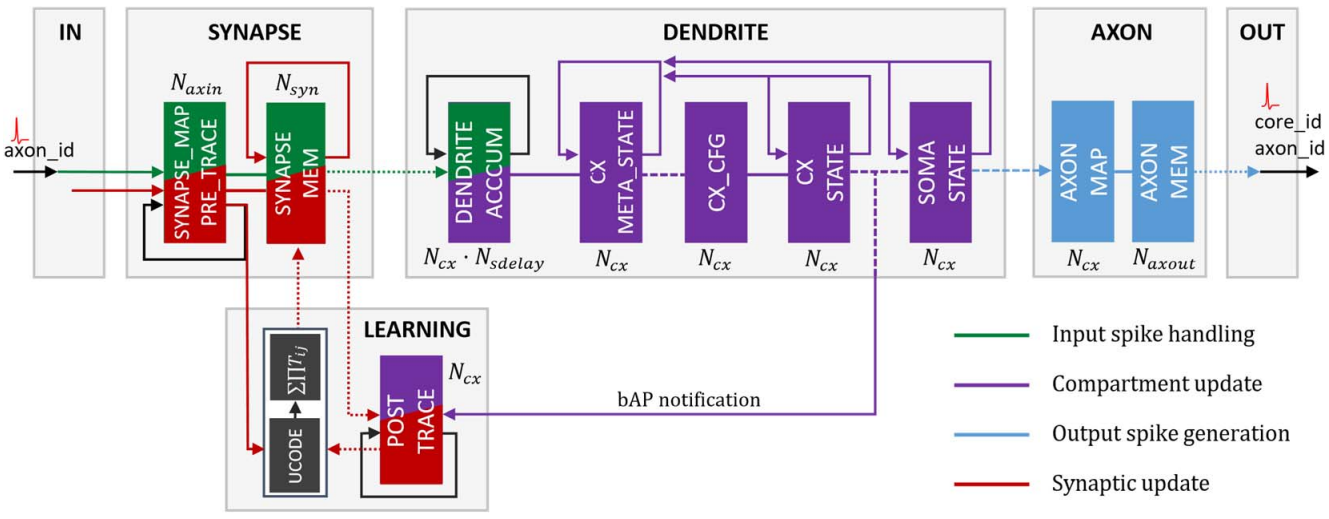
\includegraphics[width=8cm]{latex/Images/loihi_micro_architecture.png}
    \caption{Core Top-Level Microarchitecture of the Loihi chip. The SYNAPSE unit processes all incoming spikes and
    reads out the associated synaptic weights from the SRAM memory \cite{}%https://redwood.berkeley.edu/wp-content/uploads/2021/08/Davies2018.pdf
    .}
    \label{fig:loihi_micro_architecture}
\end{figure}

\subsection{Brain Adaptation}\label{subsec:brain_adaptation}
Four methods of brain adaptation are considered within this research; redundancy, reorganisation, niche construction and Timing of developmental trajectories.  Starting with redundancy, it is noted that higher vertebrate brains often have multiple neural pathways that can support certain behaviour \cite{johnson_brain_2015}. Using multiple pathways is considered a viable strategy of implementing brain adaptation in the generated SNN. However, for completeness, reorganisation and niche construction are also evaluated. Continuing with reorganisation, evidence suggests that the human brain becomes increasingly hierarchical during post-natal development \cite{supekar_brain_2013}. No levels of hierarchy are found in the generated SNN. It is noted that for more advanced applications, such as on-site learning/retraining, the increases in hierarchy of the SNN might allow for automatic recovery after radiation exposure. An example could be a pre-trained network performing re-training after passing through the Van Allen belts before arriving at another solar body. Next, niche construction has been seen in some organisms that can change the neural pathways to select environment information based on a combination of which information the organism needs and what the brain can best process \cite{johnson_brain_2015}. It is expected that including the aspect of what the brain can best process requires a highly advanced combination of objective functions and information input streams. This option is not considered feasible within this research project. Timing of developmental trajectories can be seen as a compensation mechanism that delays the development of certain brain regions such that the brain can sample information from early environments such that it can optimise its development structure \cite{johnson_brain_2015}. The timing of developmental trajectories could be applied to a Mars rover that learns object detection on Mars instead of on Earth using two different sensory inputs to provide input data and labels. If there are significant learnable differences with respect to the Earth environment, it could lead to a better trained model. In the context of the radiation robustness, the optimisation of the development structure could be used to ignore damaged neurons after radiation exposure. Redundancy is selected as primary method of brain-adaptation for the selected SNN implementation of the MDS approximation algorithm because it does not require structural hierarchies nor model training.

To see how this redundancy can be implemented the following neural coding mechanisms are evaluated:
\begin{itemize}
    \item \textit{Rate/frequency coding} - Assumes frequency or rate of action potential increases are accompanied by stimulus intensity increases.
    \item \textit{Temporal coding} - Uses high-frequency firing rate fluctuations to convey information. %Some natural frequency oscillations may be used to intelligently restructure the network using this concept.}
    \item \textit{Population coding} - Represents stimuli using combined activities of multiple neurons.% Work by fellow student Fabian Schneider at the Donders Institute showed this method in particular proved useful in the context of spiking neural network robustness. Fabian's work will be taken into account in the baseline, midterm and final phase where relevant.}
    \item \textit{Sparse coding} - Uses small subsets of neurons to encode items. %Perhaps this mechanism can be used at times to represent redundant information.}
\end{itemize}
Rate/frequency adjustments can be used to increase or lower the \textit{precision} % TODO: verify this is the correct word. 
of the spiking representation of numbers. By increasing the frequency, the relative impact of radiation induced spike omission could be reduced. % TODO: include proof of concept.
Similarly, with population coding, the population size adjustments can be used to lower the relative impact of radiation induced neuron deaths on numerical representation accuracies. No useful implementations for temporal coding and sparse coding are found in the context of radiation robustness of the generated SNN algorithm for the MDS approximation.

\subsection{Testing}\label{subsec:testing}
To test whether the brain adaptation implementations are successful, three brain adaptation implementations are compared to a baseline without brain adaptation and among each other. 

% TODO: verify subsubsections are allowed.
\subsubsection{Metrics}\label{subsubsec:metrics}
The metrics of the comparison are:
\begin{enumerate}
    \item \textit{Algorithm performance} - a score from 0 to 100\% indicating the ratio of successful solution generation on random input graphs.
    \item \textit{Neuronal \& Synaptic Overcapcity} - a score from 0 to $n$\% indicating the ratio redundant neurons and synapses with respect to the original implementation without adaptation implementation. 
    \item \textit{Energy Efficiency} - the number of spikes consumed by implementations.
    \item \textit{Time complexity} - the theoretical time complexity required for network initialisation and adaptation.
    \item \textit{Space Complexity} - the theoretical space complexity required for network initialisation and adaptation.
\end{enumerate}

\subsubsection{Simulated Radiation Damage}\label{subsubsec:simulated_radiation_damage}
The following radiation damage is simulated:
\begin{enumerate}
    \item Neuron death.
    \item Synaptic death.
    \item Neuron property changes in: $\delta u,\delta v, bias,vth$.
    \item Synaptic property changes in: $sign,weight$.
\end{enumerate}

\subsubsection{Brain Adaptation Mechanisms}\label{subsubsec:brain_adaptation_mechanisms}
The tests are performed on the following brain adaptation implementations:
\begin{enumerate}
    \item An Neumann monitoring module that scans the entire SNN network probing its behaviour, and rerouting broken neurons and/or synapses to redundant neurons.
    \item Intelligently designed redundancies of inhibited neurons that automatically take over from deceased neurons.
    \item A rate-coding frequency adaptation to reduce the relative impact of radiation induced spike ommission in a subnetwork of the complete SNN implementation of the MDS approximation.
\end{enumerate}